\documentclass[english,9pt,aspectraio=169]{beamer}
\usepackage{etex}
\usetheme{uzhneu-en-informal}
%\usepackage{uarial}
\usepackage[T1]{fontenc}
\usepackage[utf8]{inputenc}
\RequirePackage{graphicx,ae}
\usepackage{bm}
\usepackage{fancybox,amssymb,color}
\usepackage{pgfpages}
\usepackage{booktabs}
\usepackage{verbatim}
\usepackage{animate}
\usepackage{numprint}
\usepackage{dsfont}
\usepackage{tikz}
\usepackage{amsmath,natbib}
\usepackage{mathbbol}
\usepackage{babel}
\usepackage{SweaveSlides}
\usepackage{multicol}
\usepackage{xcolor}


\usetheme{uzhneu-en-informal}
\DeclareMathOperator{\po}{Poisson}
\DeclareMathOperator{\G}{Gamma}
\DeclareMathOperator{\Be}{Beta}
\DeclareMathOperator{\logit}{logit}
\def\n{\mathop{\mathcal N}}

\definecolor{Gray}{RGB}{139,137,137}
\definecolor{darkred}{rgb}{0.8,0,0}
\definecolor{Green}{rgb}{0,0.8,0.3}
\definecolor{Blue}{rgb}{0,0,1}
\def\myalert{\textcolor{darkred}}
\def\myref{\textcolor{Gray}}
\setbeamercovered{invisible}

\renewcommand{\baselinestretch}{1.2}
\beamertemplateballitem
\DeclareMathOperator{\cn}{cn} % Copy number
\DeclareMathOperator{\ccn}{ccn} % common copy number
\DeclareMathOperator{\p}{p} % common copy number
\DeclareMathOperator{\E}{E} % common copy number
\DeclareMathOperator{\given}{|} % common copy number
\def\given{\,|\,}
\def\na{\tt{NA}}
\def\nin{\noindent}
\pdfpageattr{/Group <</S /Transparency /I true /CS /DeviceRGB>>}
\def\eps{\varepsilon}

\renewcommand{\P}{\operatorname{\mathsf{Pr}}} % Wahrscheinlichkeitsmaß
\def\eps{\varepsilon}
\def\logit{\text{logit}}
%\newcommand{\E}{\mathsf{E}} % Erwartungswert
\newcommand{\Var}{\text{Var}} % Varianz
\newcommand{\NBin}{\text{NBin}}
\newcommand{\Po}{\text{Po}}
\newcommand{\N}{\mathsf{N}}

\newcommand{\hl}{\textcolor{red}}

\newcommand{\ball}[1]{\begin{pgfpicture}{-1ex}{-0.65ex}{1ex}{1ex}
\usebeamercolor[fg]{item projected}

{\pgftransformscale{1.75}\pgftext{\normalsize\pgfuseshading{bigsphere}}}
{\pgftransformshift{\pgfpoint{0pt}{0.5pt}}
\pgftext{\usebeamerfont*{item projected}{#1}}}
\end{pgfpicture}}%
\usepackage{multicol}
\newcommand{\ballsmall}[1]{\begin{pgfpicture}{-1ex}{-0.65ex}{.2ex}{.2ex}

{\pgftransformscale{1}\pgftext{\normalsize\pgfuseshading{bigsphere}}}
{\pgftransformshift{\pgfpoint{0pt}{0.5pt}}
\pgftext{\usebeamerfont*{item projected}{#1}}}
\end{pgfpicture}}%




\begin{document}

\fboxsep5pt

\frame{
\title[]{ \centering \Huge Kurs Bio144: \\
Datenanalyse in der Biologie}%\\[.3cm]
\author[Stefanie Muff, Owen L.\ Petchey]{\centering Stefanie Muff  \& Owen L.\ Petchey }
%\institute[]{Institute of Social and Preventive Medicine \\ Institute of Evolutionary Biology and Environmental Studies}
\date[]{Week 4: Multiple linear regression (finalize) / Residual analysis / Checking modelling assumptions\\ 16./17. March 2017}


\maketitle
}


\frame{\frametitle{Overview (todo: check)}
\begin{itemize}
\item Interactions between covariates
\item Multiple vs.\ many single regressions
\item Checking assumptions / Model validation 
\item What to do when things go wrong?
\item Transformation of variables/the response
\item Handling of outliers
\end{itemize}
}


\frame{\frametitle{Course material covered today}
\begin{itemize}
\item Chapter 3.3 in \emph{Lineare Regression}
\item To do
\end{itemize}
}

\frame[containsverbatim]{\frametitle{Recap of last week I}
to do 
}

\frame[containsverbatim]{\frametitle{Recap of last week I}
Last week we introduced binary and factor covariates that allowed for group-specific intercepts.
}


\frame[containsverbatim]{\frametitle{Group-specific slopes / Interactions}
It may happen that groups do not only differ in their intercept ($\beta_0$), but also in their slopes ($\beta_x$).\\[2mm]

For simplicity, let us look at a binary covariate ($x_i \in \{0,1\}$). 
}



\frame[containsverbatim]{\frametitle{}

Remember the mercury (Hg) example from last week. We now extended the dataset and include mothers \emph{and} children ($\leq 11$ years).\\[2mm]

It is known that Hg concentrations may change over the lifetime of humans. So let us look at \texttt{log(Hg$_\text{urin}$)} depending on the participants age:
\vspace{-5mm}
\begin{center}
\setkeys{Gin}{width=0.55\textwidth}
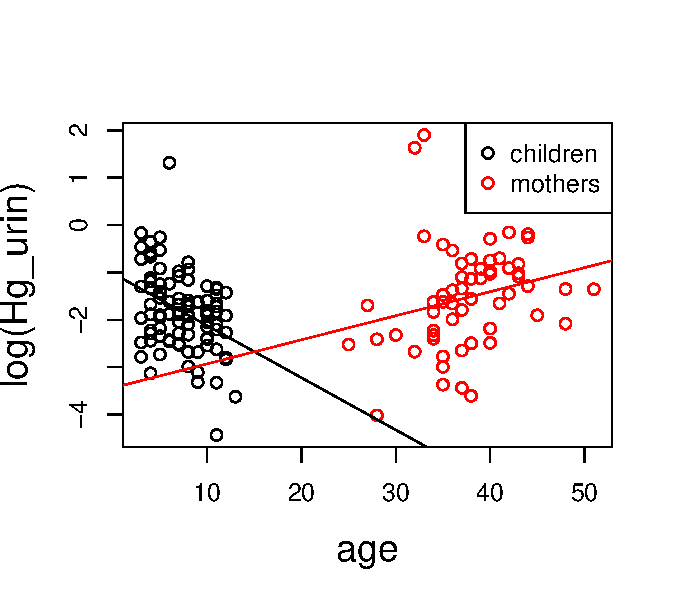
\includegraphics{Bio144_2017_week4-001}
\end{center}
An important observation is that children and mothers show different dependencies of age!
}

\frame{
It is therefore crucial to formulate a model that allows for different intercepts \emph{and} slopes, depending on group membership (mother/child).\\[2mm]

The smallest possible model is then given as\\
\begin{equation}\label{eq:HgInt}
y_i =  \beta_0 + \beta_1 \text{mother}_i + \beta_2 \text{age}_i + \beta_3\text{age}_i\cdot \text{mother}_i + e_i \ , 
\end{equation}
~\\
where $y_i=\log(Hg_{\text{urin}})_i$, and \texttt{mother} is a binary ``dummy'' variable that indicates if the person is a mother (1) or a child (0).\\[4mm]

This results in essentially {\bf two} models with group specific intercept and slope:\\[2mm]
\colorbox{lightgray}{\begin{minipage}{10cm}
Mothers ($x_i=1$): $\hat{y}_i = \beta_0 +  \beta_1 + (\beta_2 +\beta_3)\text{age}_i $  \\[2mm]
Children ($x_i=0$): $\hat{y}_i = \beta_0  + \beta_2 \text{age}_i $  
\end{minipage}}
~\\
{\scriptsize Question: why is there a hat on $\hat{y}_i$ now? Difference to $y_i$?}
}




\frame[containsverbatim]{\frametitle{}
Fitting model \eqref{eq:HgInt} in R is done as follows, where \texttt{age:mother} denotes the interaction term ($\text{age}_i\cdot \text{mother}_i$):\\[6mm]

\begin{Schunk}
\begin{Sinput}
> r.hg <- lm(log(Hg_urin)~  mother + age + age:mother,d.hg)
> summary(r.hg)$coef
\end{Sinput}
\begin{Soutput}
              Estimate Std. Error   t value     Pr(>|t|)
(Intercept) -1.0188317 0.25250071 -4.034966 8.624100e-05
mother      -2.4176907 0.91198012 -2.651034 8.874694e-03
age         -0.1101447 0.03225589 -3.414715 8.188542e-04
mother:age   0.1609032 0.03965739  4.057333 7.912112e-05
\end{Soutput}
\end{Schunk}
~\\[4mm]

Interpretation: \\[2mm]

Mothers: $\hat{y}_i = -1.02 + (-2.42) + (-0.11 + 0.16) \cdot \text{age}_i$ \\[2mm]
Children: $\hat{y}_i = -1.02  + (-0.11) \cdot \text{age}$ \\[2mm]

\begin{itemize}
\item The Hg level drops in young children.
\item The Hg level increases in adults (mothers).
\end{itemize}
}

\frame[containsverbatim]{\frametitle{}
Remember (from last week), however, that the Hg model also included smoking status, amalgam fillings and fish consumption as important predictors. It is very straightforward to just include these predictors in model \eqref{eq:HgInt}, which leads to the following model \\[6mm]

\begin{Schunk}
\begin{Sinput}
> r.hg <- lm(log(Hg_urin)~  mother * age + smoking + amalgam + fish,d.hg)
\end{Sinput}
\end{Schunk}

% latex table generated in R 3.3.2 by xtable 1.8-2 package
% Thu Jan  5 17:47:43 2017
\begin{table}[!h]
\centering
\begingroup\footnotesize
\begin{tabular}{rrrr}
  \hline
 & Coefficent & 95\%-confidence interval & $p$-value \\ 
  \hline
Intercept & -1.35 & from -1.82 to -0.87 & $<$ 0.0001 \\ 
  mother & -2.66 & from -4.38 to -0.94 & 0.003 \\ 
  age & -0.098 & from -0.16 to -0.04 & 0.001 \\ 
  smoking & 0.60 & from 0.06 to 1.15 & 0.03 \\ 
  amalgam & 0.19 & from 0.10 to 0.28 & $<$ 0.0001 \\ 
  fish & 0.072 & from 0.04 to 0.10 & $<$ 0.0001 \\ 
  mother:age & 0.14 & from 0.07 to 0.22 & 0.0001 \\ 
   \hline
\end{tabular}
\endgroup
\end{table}
{\small (Note that \texttt{mother*age} in R encodes for \texttt{mother} + \texttt{age} + \texttt{mother:age}.)}
}

\frame[containsverbatim]{
Again, for completeness, some model checking: 

\setkeys{Gin}{width=0.8\textwidth}

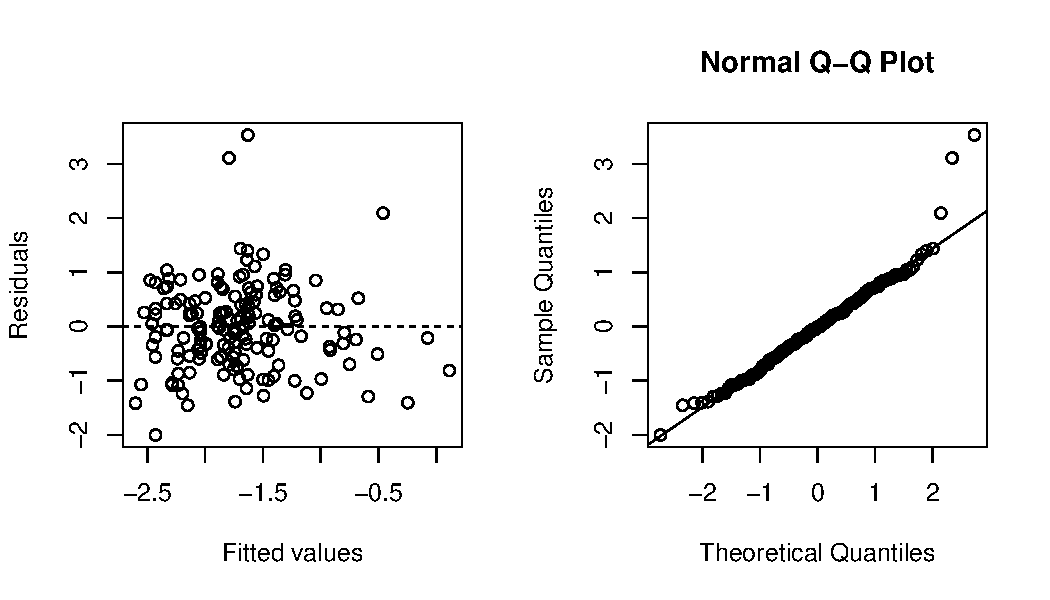
\includegraphics{Bio144_2017_week4-modelChecksHg}
}


\frame{\frametitle{Linear regression is even more powerful}
We have seen that it is possible to include continuous, binary or factorial covariates in a regression model.\\[6mm]

\colorbox{lightgray}{\begin{minipage}{10cm}
Even \alert{transformations} of covariates be included in (almost) any form. For instance, include the square of a variable $\bm{x}$
\begin{equation*}
y_i = \beta_0 + \beta_1 x_i + \beta_2 x_i^2 + e_i \ , 
\end{equation*}
which leads to a {\bf quadratic} or {\bf polynomial} regression (if higher order terms are used).
\end{minipage}}
\vspace{4mm}

Other common transformations are (see also slide \ref{sl:common}): \begin{itemize}\item $\log$ \item $\sqrt{..}$ \item $\sin$, $\cos$,... \end{itemize}
}

\frame{
How can a \emph{quadratic} regression be a \emph{linear regression}??\\[4mm]

{\bf Note}:
The word \emph{linear} refers to the \alert{linearity in the coefficients}, and not on a linear relationship between $\bm{y}$ and $\bm{x}$!\\[4mm]

\includegraphics[width=11cm]{pictures/multiplReg.pdf}
}


\frame{\frametitle{Multiple vs.\ many single regressions}
Question: I find group-specific intercepts and interactions too complicated. Could I simply fit separate models for each variable?\\[6mm]

\pause
Answer (Stahel 3.3o):\\[4mm]
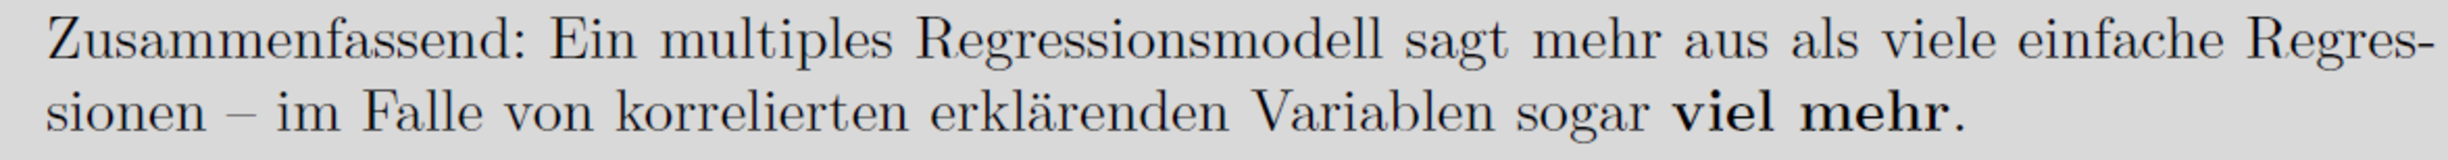
\includegraphics[width=11cm]{pictures/citation.pdf}
~\\[4mm]

Why?
}

\frame{\frametitle{Illustration}
Chapter 3.3c in the Stahel script illustrates the point on four artificial examples. The model is always given as 
\begin{equation*}
y_i = \beta_0 + \beta_1 x_i^{(1)} + \beta_2 x_i^{(2)} + e_i \  ,
\end{equation*}

where $\bm{x}^{(1)}$ is a continuous variable, and $\bm{x}^{(2)}$ is a binary grouping variable (thus taking values 0 for group 0 and 1 for group 1).\\[4mm]

Thus the model is 
\begin{equation*}
\begin{array}{lll}
\hat{y_i} &= \beta_0 +  \beta_1 x_i^{(1)} & \text{if $x_i^{(2)}=0$.} \\
\hat{y_i} &= \beta_0 + \beta_2 + \beta_1 x_i^{(1)}   & \text{if $x_i^{(2)}=1$.} 
\end{array}
\end{equation*}
}

\frame{
\includegraphics[width=11cm]{pictures/FigsAB.jpg}\\[2mm]

Example A: Within-group slope is $>0$. Fitting $y\sim x$ leads to an overestimated slope when group-variable is not included in the model.\\[4mm]

Example B: Within-group slope is $0$, but fitting $y\sim x$ leads to a slope estimate $>0$, wich is only an artefact of not accounting for the group variable $x^{(2)}$. \\[4mm]
}

\frame{
\includegraphics[width=11cm]{pictures/FigsCD.pdf}\\[2mm]

Example C: Within-group slope is $<0$, but fitting $y\sim x$ leads to an estimated slope of $>0$! \\[4mm]

Example D: Within-group slope is $<0$, but fitting $y\sim x$ leads to a slope estimate of $0$. \\[4mm]
}


\frame{\frametitle{Another interpretation of multiple regression}
In multiple regression, the coefficient $\beta_x$ of a covariate $x$ can be interpreted as follows:\\[4mm]

\colorbox{lightgray}{\begin{minipage}{10cm}
$\beta_x$ explains how the response changes with $x$, while holding all the other variables constant.
\end{minipage}}

~\\[2mm]
This idea is similar in spirit to an experimental design, where the influence of a covariate of interest on the response is investigated in various environments\footnote{Clayton, D. and M. Hills (1993). Statistical Models in Epidemiology. Oxford: Oxford University Press.}. Clayton and Hills (1993) continue (p.273):\\[3mm]

\colorbox{lightgray}{\begin{minipage}{10cm}
\begin{quote}
To extend our analogy, the data analyst is in a position like that of an experimental scientist who has the capability to plan and carry out many experiments within a single day. Not surprisingly, a cool head is required!
\end{quote}
\end{minipage}}
}

\frame{\frametitle{Checking modelling assumptions}
Remember from week 2, that in linear regression the modelling assumption is that the residuals $e_i$ are independently normally distributed around zero, that is, $e_i \sim \N(0,\sigma_e^2)$. This implies four things:\\[6mm]

\colorbox{lightgray}{\begin{minipage}{10cm}
\begin{enumerate}[a)]
\item The expected value of $e_i$ is 0: $\E(e_i)=0$.\\[2mm]
\item All $e_i$ have the same variance: $\Var(e_i)=\sigma_e^2$. \\[2mm]
\item The $e_i$ are normally distributed.\\[2mm]
\item The $e_i$ are independent of each other.
\end{enumerate}
\end{minipage}}
~\\[2mm]
So far, we have discussed the Tukey-Anscombe plot and the QQ-plot.
}

\frame{
Stahel 4.1b:
\includegraphics[width=11cm]{pictures/41b.pdf}
~\\[6mm]

The aim is to find a model that describes the data well. But always keep in mind the following statement from a wise man:\\[6mm]

\colorbox{lightgray}{\begin{minipage}{10cm}
All models are wrong, but some are useful.\\
\scriptsize{(Box 1978)}
\end{minipage}}
}

\frame{\frametitle{Overview of model-checking tools}

Those used in this course are:\\[4mm]

\begin{itemize}
\item Tukey-Anscombe plot (see weeks 2 and 3)\\
$\Rightarrow$ \myalert{To check assumptions a), b) and d)}\\[2mm]

\item Quantile-quantile (QQ) plot (see weeks 2 and 3)\\
$\Rightarrow$ \myalert{To check assumption c)}\\[2mm]


\item Scale-location plot (Streuungs-Diagramm)\\
$\Rightarrow$ \myalert{To check assumption b)}\\[2mm]

\item Leverage plot (Hebelarm-Diagramm)\\
$\Rightarrow$ \myalert{To find influential observations and/or outliers}\\[4mm]
\end{itemize}

\myalert{Note:} these four diagrams are plotted automatically by R when you use the \texttt{plot()} function on an \texttt{lm} object, for example \texttt{plot(r.hg)}.
}

\frame[containsverbatim]{\frametitle{Tukey-Anscombe plot}


It is useful to enrich the TA-plot by adding a ``running mean'' or a ``smoothed mean'', which can give hints on the trend of the residuals. For the mercury example where $\log(Hg_{\text{urin}})$ is regressed on smoking, amalgam and fish consumption for mothers only (slides 33-35 or week 3): 
\vspace{-10mm}

\begin{multicols}{2}{ll}
% \begin{center}
\setkeys{Gin}{width=0.5\textwidth}
\includegraphics{Bio144_2017_week4-hgFig}
\vspace{5mm}
~\\[1cm]
% \end{center}
The TA plot (again) indicates that there is a small problem in the range of -0.7 to -0.6, namely due to an outlier...\\
\end{multicols}

}


\frame{
We claimed that the TA plot is also able to check the \emph{independence assumption} d). But how?\\[4mm]

A dependency would be reflected by some kind of \myalert{trend}. \\[4mm]

Other ideas to plot residuals to check for a dependency? Please discuss!

}

% Todo: hide the following slide in the published version of the slides!!
\frame{
The dependency is not necessarily on the fitted values ($x$-axis of TA plot). Ideas: 
\begin{itemize}
\item Plot in dependency of time (if available) or sequence of obervations.
\item Plot against the covariates.
\end{itemize}
\begin{center}
\setkeys{Gin}{width=0.9\textwidth}
\includegraphics{Bio144_2017_week4-hgFigCov}
\end{center}
}

\frame{\frametitle{QQ-plot}

The \myalert{outlier} recorded above is also visible in the (well-known) QQ-plot, which is useful to check normal distribution of residuals (assumption c):
\begin{center}
\setkeys{Gin}{width=0.6\textwidth}
\includegraphics{Bio144_2017_week4-hgFigQQ}
\end{center}
}


\frame[containsverbatim]{
\colorbox{lightgray}{\begin{minipage}{10cm}
How do I know if a QQ-plot looks ``good''?
\end{minipage}}
\vspace{0mm}

There is no quantitative rule to answer this question, experience is needed. However, you can gain this experience from \alert{simulations}. To this end, generate the same number of data points of a normally distributed variable and compare to your plot. Example:

\begin{center}
\setkeys{Gin}{width=0.7\textwidth}
\includegraphics{Bio144_2017_week4-011}
\end{center}
}

\frame[containsverbatim]{\frametitle{Scale-location plot (Streuungs-Diagramm)}
The scale-location plot is particularly suited to check the assumption of equal variances ({\bf homoscedasticiy / Homoskedasdizit\"at}).\\[2mm]

The idea is to plot the squared residuals $\sqrt{|R_i|}$ against the fitted values $\hat{y_i}$ {\scriptsize (again using the Hg example with the mothers)}:\\[2mm]
\begin{center}
\setkeys{Gin}{width=0.6\textwidth}
\includegraphics{Bio144_2017_week4-slPlot}
\end{center}
}


\frame{\frametitle{Leverages}
To understand the leverage plot, we need to introduce the idea of the \emph{leverage} (``Hebel''), see Stahel 4.3 h).\\[2mm]

The leverage of individual $i$ is defined as $H_{ii} = (1/n) + (x_i-\overline{x})^2 SSQ^{(X)}$, which becomes larger the further away from the mean...\\[6mm]

\includegraphics[width=11cm]{pictures/leverage.jpg}

}

\frame{\frametitle{Graphical illustration of the leverage effect}
Data points with $x_i$ values far from the mean have a stronger leverage effect than when $x_i\approx \overline{x}$:

\begin{center}
\setkeys{Gin}{width=1.1\textwidth}
\includegraphics{Bio144_2017_week4-013}
\end{center}

The outlier in the middle plot ``pulls'' the regression line in its direction and biases the slope.

}

\frame[containsverbatim]{\frametitle{Leverage plot (Hebelarm-Diagramm)}
In the leverage plot, (standardized) residuals $\tilde{R_i}$ are plotted against the leverage $H_{ii}$ (continuing with the Hg example):
~\vspace{-8mm}
\begin{center}
\setkeys{Gin}{width=0.55\textwidth}
\includegraphics{Bio144_2017_week4-014}
\end{center}
{\scriptsize Note: Cook's distance measures how much the regression changes when the $i$th observation is omitted.}\\[2mm]
\myalert{Critical ranges} are the top and bottom right corners!!\\
Here, individuals 95, 101 and 106 are potential \myalert{outliers}.
}


\frame{\frametitle{What can go ``wrong'' during the modelling process?}

\begin{itemize}
\item ...
% \item Violation of assumptions:
% \begin{itemize}
% \item $\E(e_i)\neq 0$
% \item $\Var(e_i)$ not constant
% \item $e_i$ not normally distributed.
% \item Heteroscedasticity
% \end{itemize}
% \item Outliers
%
\end{itemize}
}

\frame{\frametitle{What to do when things go wrong?}
\begin{enumerate}[(i)]
\item \hl{Transform the outcome or the covariables.}\\[2mm]
\item \hl{Take care of outliers.}\\[2mm]
\item Use weighted regression (not discussed here; todo: check).\\[2mm]
\item Improve the model, e.g., by adding additional terms or interactions (see ``model selection'' in week 7).\\[2mm]
\item Use another model family (generalized or nonlinear regression model).\\[2mm]
\end{enumerate}
}


\frame[containsverbatim]{\frametitle{Transformation of the response?}
Example: Use again the mercury study, include only mothers. Use the response (Hg-concentration in the urine) \myalert{without log-transformation}. What would it look like?
\begin{Schunk}
\begin{Sinput}
> r2.urin.mother <- lm(Hg_urin ~  smoking  + amalgam + fish,data=d.hg.m)
\end{Sinput}
\end{Schunk}
\texttt{plot(r2.urin.mother)}:
\begin{center}
\setkeys{Gin}{width=0.6\textwidth}
\includegraphics{Bio144_2017_week4-016}
\end{center}
}

\frame[containsverbatim]{
Also the ``old-fashioned'' histogram of the residuals is illustrative, it is \myalert{very skewed}:
\begin{center}
\setkeys{Gin}{width=0.6\textwidth}
\includegraphics{Bio144_2017_week4-017}
\end{center}
}

\frame[containsverbatim]{
An in-summary comparison of the model with log-transformed response:

\begin{center}
\setkeys{Gin}{width=0.6\textwidth}
\includegraphics{Bio144_2017_week4-019}
\end{center}
This looks {\bf much} better! However... there is this individual 106 that needs some closer inspection (see slide \ref{sl:outliersHg} for the solution regarding this outlier).
}


\frame{
A similar example is given in Stahel 4.4 a+b. The diagnostic plots of a regression where the log-transformation of the outcome was forgotten looked like this:\\
\begin{center}
\includegraphics[width=8cm]{pictures/logT.pdf}
\end{center}
}

\frame{\frametitle{Common transformations}\label{sl:common}
Which tranformations should be considered to cure model deviation symptoms? Answering this depends on plausibility and simplicity, and requires some experience. \\[6mm]

The most common and useful \myalert{first aid transformations} are:\\[4mm]

\colorbox{lightgray}{\begin{minipage}{10cm}
\begin{itemize}
\item The log transformation for {\bf concentrations} and {\bf absolute values}.
\item The square-root ($\sqrt{\cdot}$) transformation for {\bf count data}.
\item The $\arcsin(\sqrt{\cdot})$ transformation for {\bf proportions/percentages}.
\end{itemize}
\end{minipage}}
~\\[4mm]

These transformations can (or should) also be applied on covariates!
}

\frame[containsverbatim]{\label{sl:hgSqrt}
For instance, the number of amalgam fillings and the number of monthly fish meals should be sqrt-transformed in the mercury example:
\begin{Schunk}
\begin{Sinput}
> r4.urin.mother <- lm(log10(Hg_urin) ~  smoking + sqrt(amalgam) + sqrt(fish),data=d.hg.m)
\end{Sinput}
\end{Schunk}
\begin{center}
\setkeys{Gin}{width=0.65\textwidth}
\includegraphics{Bio144_2017_week4-hgFig}
\end{center}
}

\frame[containsverbatim]{\frametitle{Outliers}
{\scriptsize (See Stahel chapter 4.5)}\\
The above plots illustrate that outliers are visible in all diagnostic plots. \\[4mm]

What to do in this case?

\begin{enumerate}
\item Start by checking the correctness of the data. Is there a typo or a digital point that was shifted by mistake? Check the covariates and the response.\\[2mm]
\item If not, ask whether the model has been misspecified. Do reasonable transformations of the response or the covariables eliminate the outlier? Have the residuals a distribution with a long tail (which makes it more likely that extreme observations occur)?\\[2mm]
\item Sometimes, an outlier may be the most interesting observation in a dataset!\\[2mm]
\item Consider that outliers can also occur by chance!
\end{enumerate}

}

\frame{\frametitle{Deleting outliers?}
It might seem tempting to delete observations that apparently don't fit into the picture. However:\\[4mm]

\begin{itemize}
\item Do this {\bf only with absolute care}, e.g., if an observation has extremely implausible values! \\[2mm]
\item Before deleting outliers, check points 1-4 from the previous slide. \\[2mm]
\item When deleting outliers or the x\% of most extreme observations, you {\bf must mention this in your report}. \\[2mm]
\item Confidence intervals, tests and $p$-values might be biased.
\end{itemize}


}


\frame[containsverbatim]{\frametitle{The outlier in the Hg study}\label{sl:outliersHg}
In the Hg study, it turned out later on that the outlier 106 had five unreported amagam fillings! \\[2mm]
A corrected analysis gives a much more regular picture (please compare to slide \ref{sl:hgSqrt}):
\vspace{-4mm}

\begin{center}
\setkeys{Gin}{width=0.6\textwidth}
\includegraphics{Bio144_2017_week4-hgFigOut}
\end{center}

}

\frame{\frametitle{Summary}
Ev use ``Merkpunkte'' from Stahel slides (slide 41). What was today's lecture all about?
}
% \frame{References:
% \bibliographystyle{Chicago}
% \bibliography{refs}
% }



\end{document}
